\section{FuD-BOINC}

\begin{subsection}{¿Qué es FuD-BOINC?}

	\begin{frame}\frametitle{¿Qué es FuD-BOINC?}	
		\begin{itemize}
		\item Una nueva implementación de la capa L1 de \fud .
		\item Permite que aplicaciones desarrolladas con \fud \ puedan correr sobre proyectos BOINC.
		\item Permite abstraer al desarrollador de aplicaciones \fud \ de la API de BOINC.
		\end{itemize}
		
		\begin{center}
			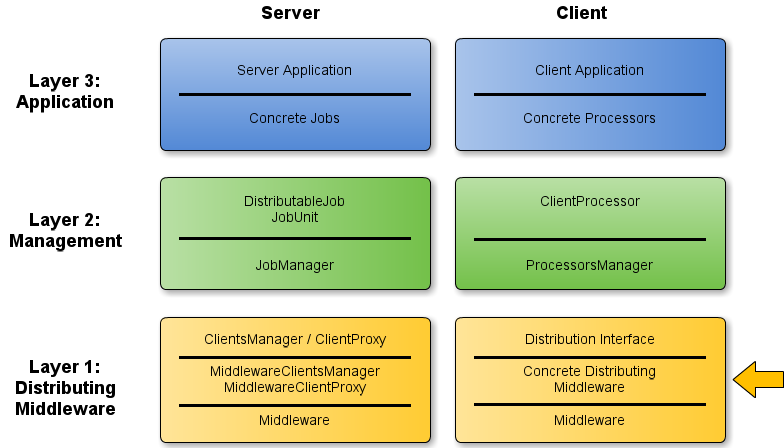
\includegraphics[scale=0.27]{images/AbstractLayers-FuD-L1.png}
		\end{center}
	\end{frame}
	
\end{subsection}
				

\begin{subsection}{Diseño}

	\begin{frame}\frametitle{Capa de distribución: lado servidor}
		\begin{center}
			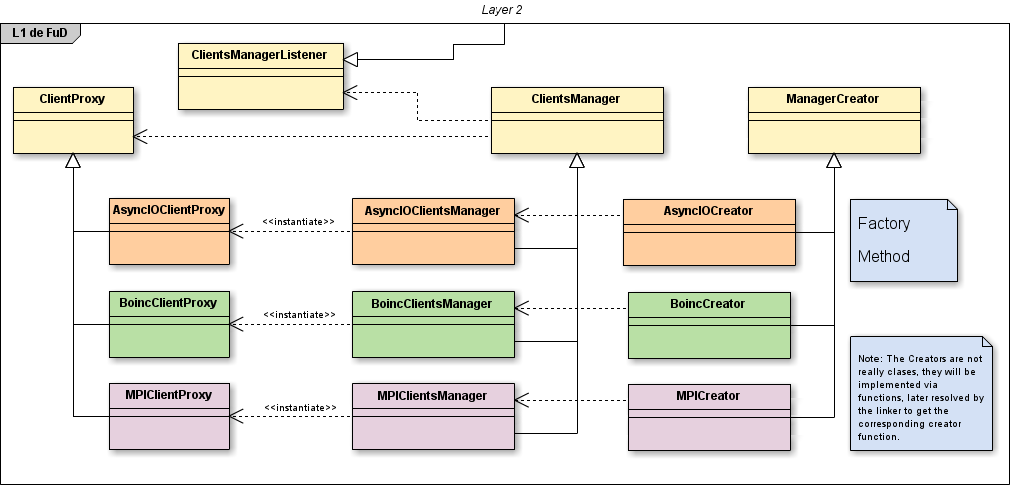
\includegraphics[scale=0.31]{images/diseno-servidor-fud.png}
		\end{center}
	\end{frame}
	
	\begin{frame}\frametitle{Lado servidor: \texttt{BoincClientsManager}}
  		\begin{figure}[h]
    		\begin{minipage}{3.3cm}
      			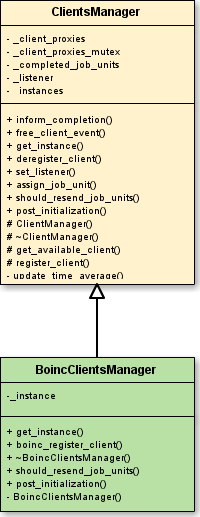
\includegraphics[scale=0.35]{images/BoincClientsManager.png}
    		\end{minipage}
    		\begin{minipage}{0.67 \textwidth}
				\begin{block}{\texttt{BoincClientsManager}}
      				Hereda de la clase \texttt{ClientsManager} de \fud .
      			\end{block}
      			\vspace{7mm}
      			\begin{block}{Responsabilidades}
      				\begin{itemize}
						\item Realizar el registro de un único cliente.
						\item Comunicar al manejador de trabajos la disponibilidad del cliente conectado.
					\end{itemize}
      			\end{block}	
      		\end{minipage}
    	\end{figure}
	\end{frame}
	
	\begin{frame}\frametitle{Lado servidor: \texttt{BoincClientProxy}}
  		\begin{figure}[h] 		
    		\begin{minipage}{2.7cm}
      			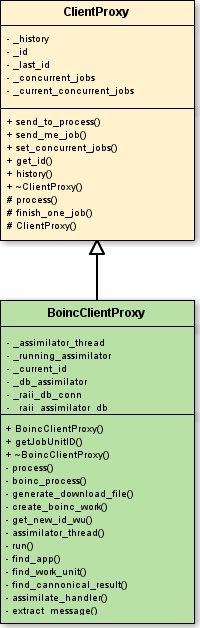
\includegraphics[scale=0.3]{images/BoincClientProxy.png}
    		\end{minipage}
    		\begin{minipage}{0.7 \textwidth}
      			\begin{block}{\texttt{BoincClientProxy}}
      				Hereda de la clase \texttt{ClientProxy} de \fud \ y representa un cliente conectado con la 
      				particularidad que siempre está disponible.
      			\end{block}
				\vspace{3mm}
      			\begin{block}{Responsabilidades}
      				\begin{itemize}
						\item Mantener una conexión directa con la base de datos del proyecto BOINC.
						\item Generar un trabajo de BOINC a partir de una \texttt{JobUnit}.
						\item Obtener los resultados enviados por los clientes e informarlos a L2.
					\end{itemize}
      			\end{block}	
      		\end{minipage}
    	\end{figure}
	\end{frame}

	\begin{frame}\frametitle{Capa de distribución: lado cliente}
		\begin{center}
			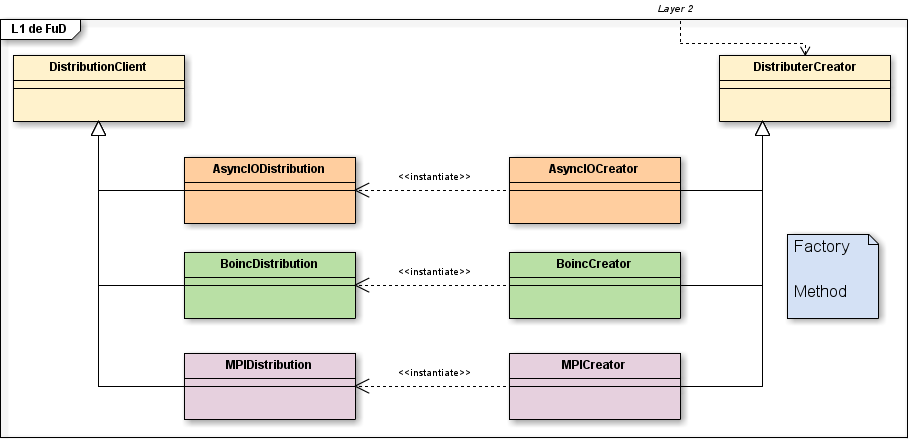
\includegraphics[scale=0.35]{images/diseno-cliente-fud.png}
		\end{center}
	\end{frame}

	\begin{frame}\frametitle{Lado cliente: \texttt{BoincDistribution}}
  		\begin{figure} 		
    		\begin{minipage}{0.2\linewidth}
      			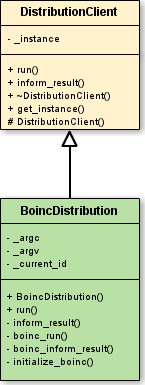
\includegraphics[scale=0.5]{images/BoincDistribution.png}
    		\end{minipage}
    		\hfill
    		\begin{minipage}{0.7\linewidth}
      			\begin{block}{\texttt{BoincDistribution}}
      				Hereda de la clase DistributionClient de \fud \ y provee la funcionalidad necesaria para que la aplicación pueda correr 					satisfactoriamente sobre el cliente BOINC.
      			\end{block}
				\vspace{2mm}
      			\begin{block}{Responsabilidades}
      				\begin{itemize}
      					\item Extraer la \texttt{JobUnit} del archivo de entrada brindado por el \textbf{cliente de BOINC}.
						\item Envíar la \texttt{JobUnit} a la capa L2 para su procesamiento.
						\item Escribir el resultado de la tarea en un archivo de salida para que el \textbf{cliente de BOINC} 
						lo informe al servidor.
					\end{itemize}
      			\end{block}	
      		\end{minipage}
    	\end{figure}
	\end{frame}

\end{subsection}


\begin{subsection}{Implementación}

	\begin{frame}[fragile]\frametitle{API de BOINC}
		\begin{block}{Servidor}
			Del lado servidor de FuD-BOINC se debió utilizar la API de BOINC para realizar las siguientes tareas:
			\vspace{1mm}
			\begin{itemize}
				\item Leer el archivo de configuración del proyecto BOINC:
					\begin{lstlisting}
						config.parse_file()
					\end{lstlisting}
				\item Establecer una conexión con la base de datos:
					\begin{lstlisting}
						boinc_db.open(config.db_name, config.db_host, config.db_user, config.db_passwd);
					\end{lstlisting}
			\end{itemize}
		\end{block}
	\end{frame}

	\begin{frame}[fragile]\frametitle{API de BOINC}
		\begin{block}{Cliente}
			Del lado cliente de FuD-BOINC se debió utilizar la API de BOINC para realizar las siguientes tareas:
			\vspace{2mm}
			\begin{itemize}
				\item Inicializar los diagnósticos de BOINC:
					\begin{lstlisting}
						int boinc_init_diagnostics(int flags);
					\end{lstlisting}
				\item Inicializar la aplicación cliente de BOINC para que sea propiamente ejecutada por el cliente de BOINC:
					\begin{lstlisting}
						boinc_init();
          			\end{lstlisting}
				\item Finalizar la aplicación cliente de BOINC:
         			\begin{lstlisting}
						int boinc_finish(int status);
          			\end{lstlisting}
    		\end{itemize}
  		\end{block}
	\end{frame}

	\begin{frame}\frametitle{Servidor: envío de trabajos}
		\begin{block}{}
			\fud \ provee el método \texttt{process()} mediante el cual se envían \texttt{JobUnits} a clientes.
		\end{block}
		\vspace{5mm}
		\pause
		En FuD-BOINC, el método \texttt{process()} se encarga de traducir una \texttt{JobUnit} a un trabajo de BOINC
		mediante los siguientes pasos:
		\vspace{5mm}
		\begin{enumerate}
		\addtolength{\itemsep}{2mm}
			\item Serializar la \texttt{JobUnit} de \fud \ dentro de un archivo binario.
			\item Leer la plantilla utilizada por BOINC en donde se especifican las características de la \textbf{workunit} a crear.
			\item Invocar al método \texttt{create\_boinc\_work()}.
		\end{enumerate}
	\end{frame}

	\begin{frame}[fragile]\frametitle{Servidor: crear trabajo de BOINC}
		\begin{block}{create\_boinc\_work()}
			El método \texttt{create\_boinc\_work()} es el encargado de crear un nuevo trabajo de BOINC.
		\end{block}
		Las tareas llevadas a cabo por éste método se pueden simplificar en los siguientes pasos:
		\begin{enumerate}
			\item Crear el nombre que identifica la \textbf{workunit}.
			\item Asociar la nueva tarea a la aplicación en ejecución.
			\item Crear el trabajo invocando al método \texttt{create\_work()} de BOINC.
		\end{enumerate}
		\vspace{2mm}
		\begin{lstlisting}[frame=single]   
			create_work( wu, wu_template,
			             RE_TEMPLATE.c_str(),
			             config.project_path(RE_TEMPLATE.c_str()),
			             input_files, NRO_INFILES, config );
		\end{lstlisting}
	\end{frame}

	\begin{frame}\frametitle{Servidor: obtener resultados de clientes}
		\begin{block}{}
			\fud \ provee el método \texttt{inform\_completion()} para informar los resultados de las \texttt{JobUnit} 
			recibidos desde los clientes a las capas superiores.
		\end{block}
		\vspace{2mm}
		\pause
		\begin{block}{}
			Para recibir y manejar los resultados enviados por los clientes de BOINC, se debió integrar 
			el comportamiento del demonio \textit{\textbf{assimilator}} como parte del comportamiento de FuD-BOINC.
		\end{block}
		\vspace{2mm}
		\pause
		\begin{block}{¿Cómo?}
			Se implementó un nuevo hilo de ejecución dentro del servidor FuD-BOINC para que se encargue de chequear 
			la existencia de nuevos resultados no asimilados.
		\end{block}
	\end{frame}

	\begin{frame}[fragile]\frametitle{Servidor: asimilador de tareas}
		\begin{block}{}
			El thread assimilator cumple con las siguientes funciones:
			\vspace{2mm}
			\begin{itemize}
				\item Buscar en la base de datos workunits no asimiladas
				\item Verificar si se encontró resultado canónico para dichas workunits
				\item Invocar al método \texttt{assimilate\_handler()}, una vez confirmada la existencia de un resultado canónico
			\end{itemize}
		\end{block}
		\pause
		\vspace{4mm}
		\begin{block}{assimilate\_handler()}
			Extrae el resultado de la workunit del archivo de salida enviado por el cliente BOINC para luego informarlo 
			mediante el método \texttt{inform\_completion()} de FuD.
		\end{block}
	\end{frame}

	\begin{frame}[fragile]\frametitle{Servidor: asimilador de tareas}
		\textbf{Ciclo del \texttt{assimilator\_thread()}:}
		\begin{lstlisting}
	app = find_app(NAME_APP, _db_assimilator);
	while(_running_assimilator)
	{
	    if (find_work_unit(app, wu) == true)
	    {
	        if ( find_cannonical_result(wu,canonical_result) == true )
	        {
	            assimilate_handler(wu,canonical_result);
	            update_wu_state(wu, WuDone);
	        }
	     }
	     sleep(SLEEP_INTERVAL);
	}
		\end{lstlisting}
		\textbf{Tareas más relevantes del método \texttt{assimilate\_handler()}:}
		\begin{lstlisting}
			std::string* msg = extract_message(output_file);
			ClientsManager::get_instance()->inform_completion(getJobUnitID(), msg);
		\end{lstlisting}
	\end{frame}

	\begin{frame}\frametitle{Cliente: computación de una tarea}
		\begin{block}{}
			\fud \ provee el método \texttt{run()} el cual debe ser implementado con las tareas específicas que debe 
			realizar el cliente para llevar a cabo el cómputo de las JobUnits.
		\end{block}
		\pause
		\vspace{4mm}
		En FuD-BOINC, el método \texttt{run()} se remite a obtener la \texttt{JobUnit} de \fud \ a partir del trabajo 
		de BOINC mediante los siguientes pasos:
		\vspace{4mm}
		\begin{enumerate}\addtolength{\itemsep}{2mm}
		    \item Leer el archivo binario que contiene encapsulada la JobUnit de FuD
		    \item Extraer el mensaje correspondiente a la JobUnit de FuD
		    \item Invocar al método \texttt{deliver\_message()} quien enviará el contenido a las capas superiores para su computación.
		\end{enumerate}
	\end{frame}

	\begin{frame}\frametitle{Cliente: informar resultado}
		\begin{block}{}
			\fud \ provee el método \texttt{inform\_result()} cuya función es enviar el resultado de la computación al servidor.
		\end{block}
		\pause
		\vspace{6mm}
		En FuD-BOINC se remite a invocar al método \texttt{boinc\_inform\_result()} el cual se encarga de las siguientes tareas:
		\vspace{4mm}
		\begin{enumerate}\addtolength{\itemsep}{3mm}
			\item Obtener el resultado de la computación
			\item Escribir dicho resultado en un archivo de salida asociado al trabajo de BOINC
		\end{enumerate}
	\end{frame}

	\begin{frame}[fragile]\frametitle{Cliente: informar resultado}
		Parte del código de \texttt{boinc\_inform\_result()}:
		\vspace{4mm}
			\begin{lstlisting}
		std::string body = ProcessorsManager::get_instance()->get_return_message();
	
		OutputMessage bos;
		bos << _current_id << body;
	
		// File to upload to server.
		std::ofstream out;
	
		//enable the exceptions
		out.exceptions ( std::ofstream::failbit | std::ofstream::badbit );
		out.open(file_name.c_str(), std::ios::binary);
	
		// Get the message with result of computation to send back to server
		out << bos.str();
			\end{lstlisting}
	\end{frame}

	\begin{frame}\frametitle{Cliente: compilación en Windows}
		\begin{block}{}
			Fue necesario compilar el cliente de FuD-BOINC para sistemas operativos Windows ya que actualmente son los más utilizados.
		\end{block}
		\begin{block}{}
			Pasos para la compilación:
			\vspace{2mm}
			\begin{enumerate}\addtolength{\itemsep}{1mm}
				\item Compilar las librerías BOINC.
				\item Generar y configurar un proyecto solución de \textit{Visual Studio} para la compilación de FuD-BOINC.
				\item Resolver dependencias con las librerías: boost, pthread, mili y MySQL
				\item Modificar el tipo de \texttt{include} realizado en algunos archivos del cliente \fud.
				\item Compilar el cliente de \fud.
			\end{enumerate}		
		\end{block}
	\end{frame}

\end{subsection}


\begin{subsection}{Interacción entre FuD y BOINC}

	\begin{frame}\frametitle{Servidor: envío de una \texttt{JobUnit}}
		\begin{center}
			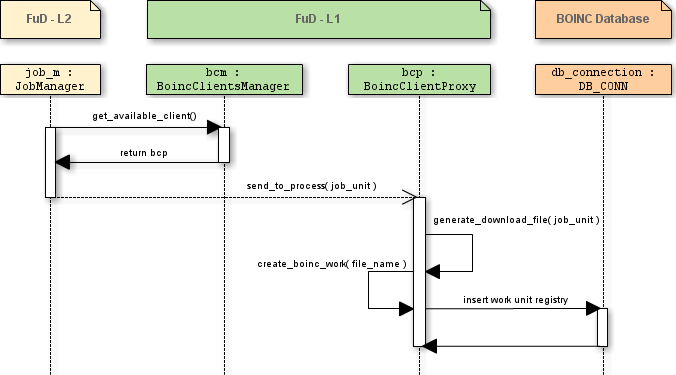
\includegraphics[scale=0.45]{images/interaccion-fud-boinc-server_side.png}
		\end{center}
	\end{frame}
	
	\begin{frame}\frametitle{Cliente: computación de una \texttt{JobUnit}}
		\begin{center}
			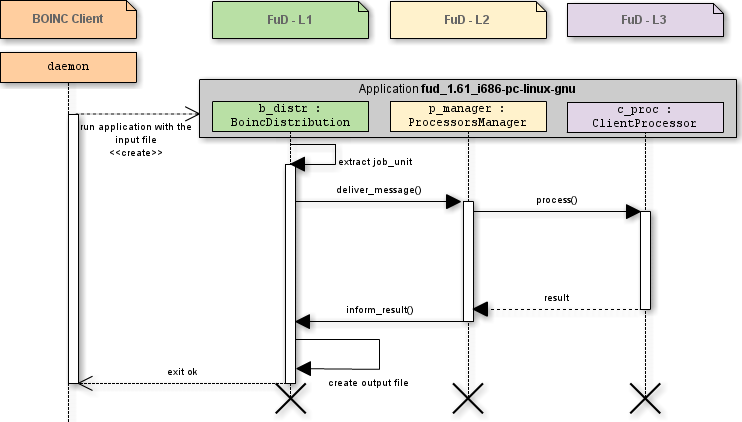
\includegraphics[scale=0.4]{images/interaccion-fud-boinc-client_side.png}
		\end{center}
	\end{frame}

\end{subsection}

